\documentclass[dvipsnames, tikz]{standalone}
\usepackage{amsmath}
\usepackage{arevmath}
\usepackage{xcolor}
\usepackage{tikz}
\usetikzlibrary{calc}
\usetikzlibrary{decorations.pathreplacing,calligraphy,3d}
\usetikzlibrary{matrix,shapes,fit,backgrounds}

\begin{document}
	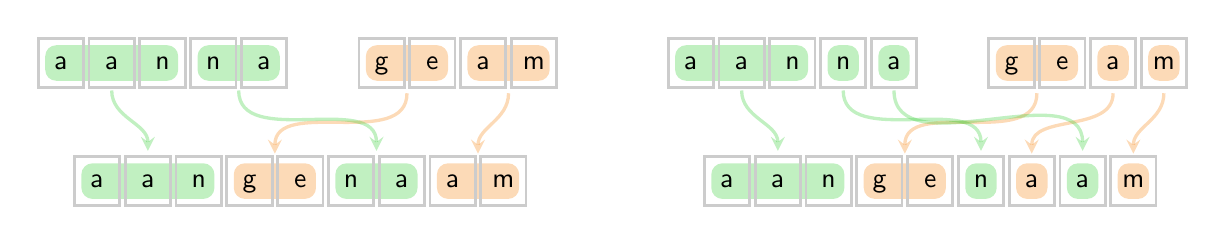
\begin{tikzpicture}[
		%Global config
		>=latex,
		line width=1pt,
		color = black,
		every left delimiter/.style={xshift=1ex},
		every right delimiter/.style={xshift=-1ex},
		%Styles
		Vector/.style={
			matrix of nodes,
			text height=1.85ex,
			text depth=0.75ex,
			text width=2.25ex,
			align=center,
			%left delimiter=(,
			%right delimiter=),
			column sep=1pt,
			row sep=1pt,
			nodes={draw=black!20}, % Uncoment to see the square nodes.
			%nodes in empty cells,
		},
		Matrix/.style={
			matrix of nodes,
			%text height=2.5ex,
			%text depth=0.75ex,
			%text width=3.25ex,
			%align=center,
			left delimiter=(,
			right delimiter=),
			%column sep=1pt,
			%row sep=1pt,
			%nodes={draw=black!10}, % Uncoment to see the square nodes.
			%nodes in empty cells,
		},
		DA/.style={
			fill,
			opacity=0.3,
			rounded corners,
			inner sep=-3pt,
			line width=1pt,
		},
		DG/.style={
			%line cap = round,
			%rounded corners=0.25ex,
			line width = 16pt,
			opacity = 0.3,
		}
		]
		
		\matrix[Vector] at (3.75,0) (M){ % Matrix contents  
			\sf g & \sf e & \sf a & \sf m\\
		};
		
		\matrix[Vector] at (0,0) (N){ % Matrix contents  
			\sf a & \sf a & \sf n & \sf n & \sf a\\
		};
	
		\matrix[Vector] at (1.75,-1.5) (O){ % Matrix contents  
			\sf a & \sf a & \sf n & \sf g & \sf e & \sf n & \sf a & \sf a & \sf m\\
		};
	
		\begin{scope}[on background layer] 
			%To delimit internal area groups
			%\node[DA,blue,fit=(M-3-2)(M-5-4)](subM-2){};
			\node[DA,LimeGreen,fit=(N-1-1)(N-1-3)](A1){};
			\node[DA,LimeGreen,fit=(O-1-1)(O-1-3)](C1){};
			
			\node[DA,BurntOrange,fit=(M-1-1)(M-1-2)](B1){};
			\node[DA,BurntOrange,fit=(O-1-4)(O-1-5)](C2){};
			
			\node[DA,LimeGreen,fit=(N-1-4)(N-1-5)](A2){};
			\node[DA,LimeGreen,fit=(O-1-6)(O-1-7)](C3){};
			
			\node[DA,BurntOrange,fit=(M-1-3)(M-1-4)](B2){};
			\node[DA,BurntOrange,fit=(O-1-8)(O-1-9)](C4){};
			
			% For line sectors		
			\draw[LimeGreen, very thick, -stealth, opacity=0.3] ([yshift=-3pt]A1.south) to[out=-90, in=90] ([yshift=4pt]C1.north);   
			\draw[BurntOrange, very thick, -stealth, opacity=0.3] ([yshift=-4pt]B1.south) to[out=-90, in=90]  ([yshift=3pt]C2.north);   
			\draw[LimeGreen, very thick, -stealth, opacity=0.3] ([yshift=-3pt]A2.south) to[out=-90, in=90]  ([yshift=4pt]C3.north);   
			\draw[BurntOrange, very thick, -stealth, opacity=0.3] ([yshift=-4pt]B2.south) to[out=-90, in=90]  ([yshift=3pt]C4.north);   
		\end{scope}
	
		\begin{scope}[xshift=8cm]
			\matrix[Vector] at (3.75,0) (A){ % Matrix contents  
				\sf g & \sf e & \sf a & \sf m\\
			};
			
			\matrix[Vector] at (0,0) (B){ % Matrix contents  
				\sf a & \sf a & \sf n & \sf n & \sf a\\
			};
			
			\matrix[Vector] at (1.75,-1.5) (C){ % Matrix contents  
				\sf a & \sf a & \sf n & \sf g & \sf e & \sf n & \sf a & \sf a & \sf m\\
			};
			
			\begin{scope}[on background layer] 
				%To delimit internal area groups
				%\node[DA,blue,fit=(M-3-2)(M-5-4)](subM-2){};
				\node[DA,LimeGreen,fit=(B-1-1)(B-1-3)](AA1){};
				\node[DA,LimeGreen,fit=(C-1-1)(C-1-3)](CC1){};
				
				\node[DA,BurntOrange,fit=(A-1-1)(A-1-2)](BB1){};
				\node[DA,BurntOrange,fit=(C-1-4)(C-1-5)](CC2){};
				
				\node[DA,LimeGreen,fit=(B-1-4)(B-1-4)](BB2){};
				\node[DA,LimeGreen,fit=(C-1-6)(C-1-6)](CC3){};
				
				\node[DA,BurntOrange,fit=(A-1-3)(A-1-3)](AA2){};
				\node[DA,BurntOrange,fit=(C-1-7)(C-1-7)](CC4){};
				
				\node[DA,LimeGreen,fit=(B-1-5)(B-1-5)](BB3){};
				\node[DA,LimeGreen,fit=(C-1-8)(C-1-8)](CC5){};
				
				\node[DA,BurntOrange,fit=(A-1-4)(A-1-4)](AA3){};
				\node[DA,BurntOrange,fit=(C-1-9)(C-1-9)](CC6){};
				
				% For line sectors		
				\draw[LimeGreen, very thick, -stealth, opacity=0.3] ([yshift=-3pt]AA1.south) to[out=-90, in=90] ([yshift=4pt]CC1.north);   
				\draw[BurntOrange, very thick, -stealth, opacity=0.3] ([yshift=-4pt]BB1.south) to[out=-90, in=90]  ([yshift=3pt]CC2.north);   
				\draw[LimeGreen, very thick, -stealth, opacity=0.3] ([yshift=-3pt]BB2.south) to[out=-90, in=90]  ([yshift=4pt]CC3.north);   
				\draw[BurntOrange, very thick, -stealth, opacity=0.3] ([yshift=-4pt]AA2.south) to[out=-90, in=90]  ([yshift=3pt]CC4.north); 
				\draw[LimeGreen, very thick, -stealth, opacity=0.3] ([yshift=-3pt]BB3.south) to[out=-90, in=90]  ([yshift=4pt]CC5.north);   
				\draw[BurntOrange, very thick, -stealth, opacity=0.3] ([yshift=-4pt]AA3.south) to[out=-90, in=90]  ([yshift=3pt]CC6.north); 
			\end{scope}
		\end{scope}
		
	\end{tikzpicture}
\end{document}